\documentclass[aps,prl,preprint]{revtex4}
\usepackage{bm}
\usepackage{enumitem}
\usepackage{graphicx}
\usepackage[colorlinks]{hyperref}

\begin{document}

\title{Simple Tight-Binding Model on Triangular Lattice}

\author{Shi Wang}

\affiliation{National Laboratory of Solid State Microstructures and Department of Physics, Nanjing University, Nanjing 210093, China}

\date{\today}

\maketitle

\section{The model definition}

The simple tight-binding model on the triangular lattice is defined as fellow:
\begin{itemize}[leftmargin=2cm]
    \item Only nearest-neighbor hopping is considered
    \item No spin-flip hopping is involved
    \item Only one orbit and two spin flavors(spin-up and spin-down) are involved on every lattice site
\end{itemize}

The model Hamiltonian:
\begin{equation}
    H = -t \sum_{<ij>\alpha} c_{i\alpha}^{\dagger} c_{j\alpha} + \mu \sum_{i\alpha} c_{i\alpha}^{\dagger} c_{i\alpha}
\end{equation}
where $<ij>$ stands for nearest-neighbor and $\alpha$ correspond to spin-up and spin-down.

The resulting dispersion relation is:
\begin{equation}
    E_{\bm{k}} = \mu - 2t (\cos \bm{k} \cdot \bm{r}_{1} + \cos \bm{k} \cdot \bm{r}_{2} + \cos \bm{k} \cdot \bm{r}_{3})
\end{equation}

\section{The basic aspects}

The basic aspects of this model is shown in Fig.~\ref{fig:BasicsOfTriangleSimpleTB}.
\begin{figure}[h]
    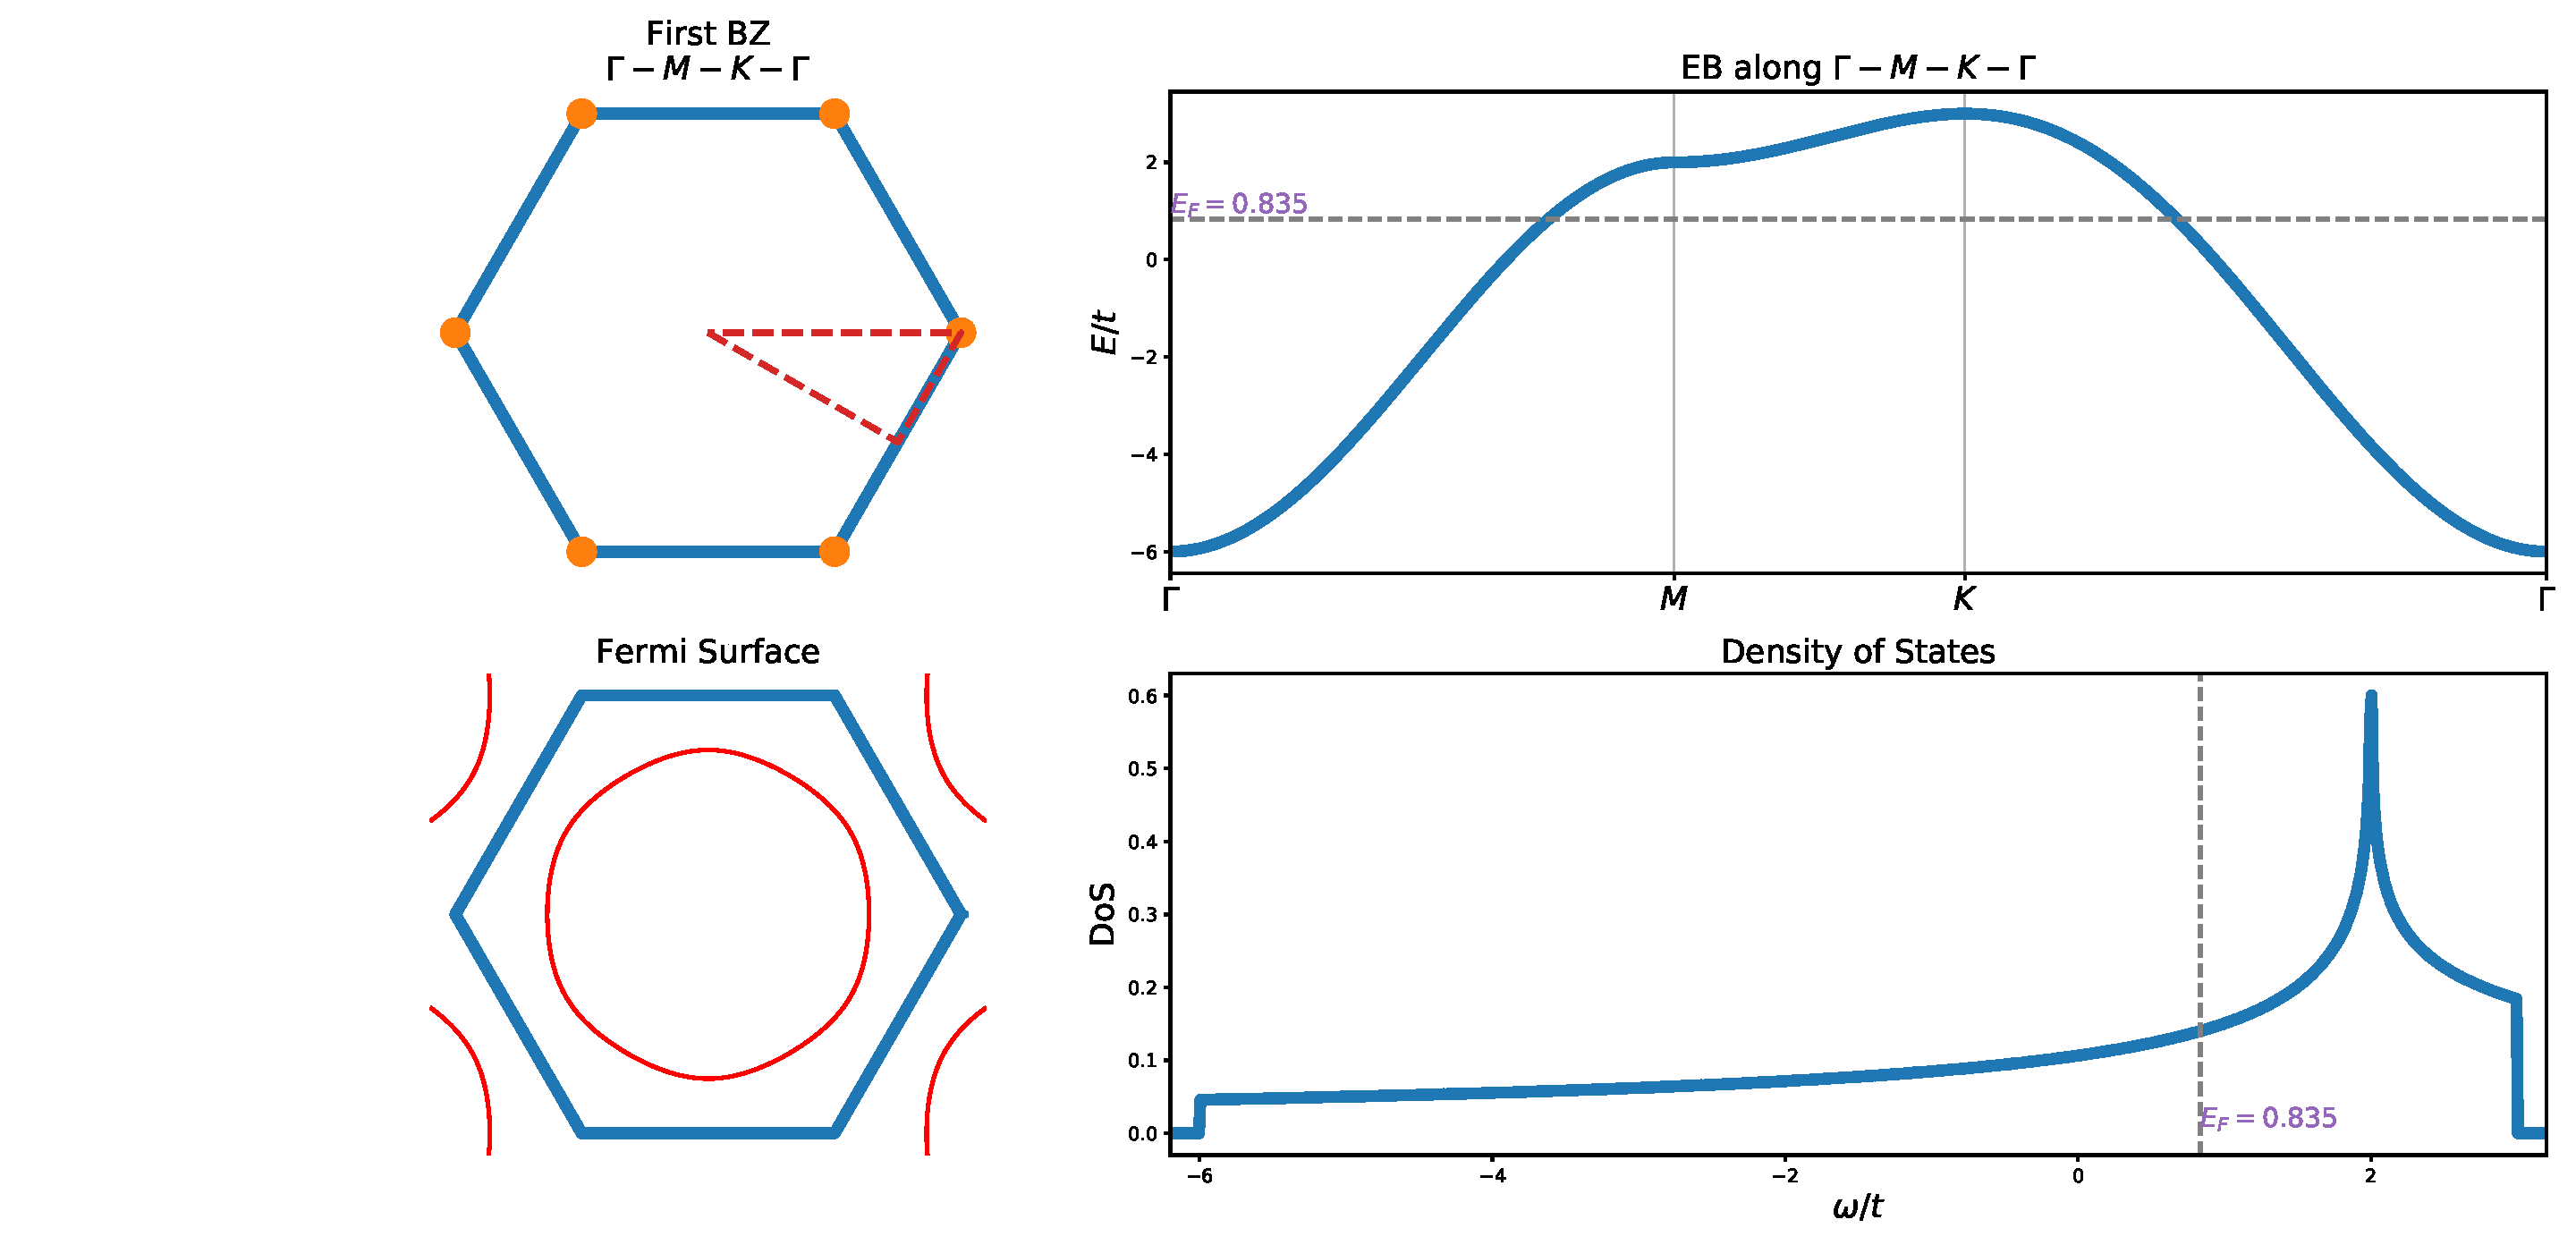
\includegraphics[width=0.9\textwidth]{BasicsOfTriangleSimpleTB.pdf}
    \caption{\label{fig:BasicsOfTriangleSimpleTB}The basic aspects of the tight-binding model.}
\end{figure}

\end{document}
